\RequirePackage[l2tabu, orthodox]{nag}
\documentclass[11pt, a4paper]{article}

\usepackage[colorlinks, debug]{packages/preambule}  

% explications :
% - https://en.wikibooks.org/wiki/LaTeX/Glossary

% \newglossaryentry{<label>}{
%	 name = {<nom>},
%	 description = {<description>},
%	 first = {<premier appel>},
%	 plural = {<si on ajoute pas de 's' à la fin>},
%	 symbol = {<symbole pi>},
% 	 see = {<label_a_voir},
% }

% \newacronym{<label>}{<abbreviation>}{<full>}
% \newacronym[longplural={pluriel}]{<label>}{<abbreviation>}{<full>}


% utilisation (pour tout):
% - \gls(<label>)
% - \Gls(<label>)  		=> avec majuscule
% - \glspl(<label>)  	=> pluriel
% - \Glspl(<label>)		=> pluriel avec majuscule
% - \glsdesc{<label>}  	=> affiche la description
% - \glssymbol{<label>}	=> affiche le symbole

% utilisation en plus pour les accronymes : 
% - \acrshort{<label>}	=> donne l'abbréviation
% - \acrlong{<label>}	=> donne la description "full"
% - \acrfull{<label>}	=> donne "full (abbreviation)"



\newglossaryentry{mot}{
	name=mot,
	description={un mot},
	first={le premier mot (mot)}
}
 
\addbibresource{bibliographie/bibliographie.bib} 
% https://en.wikibooks.org/wiki/LaTeX/Bibliography_Management#biblatex


\begin{document}

\pagenumbering{roman} 	% numérotation .i, .ii, .iii
\pagestyle{empty}		% pas de header / footer


\begin{titlepage}	% Pour réaliser une page de couverture

\begin{center}



% images en haut de page
\begin{minipage}[t]{0.48\textwidth}
	\begin{flushleft}
		
\includegraphics [width=60mm]{images/logo_ecoles/Polytech_Nantes_Universite} \\
	\end{flushleft}
\end{minipage}
\begin{minipage}[t]{0.48\textwidth}
	\begin{flushright}
		
\includegraphics [width=50mm]{images/logo_ecoles/Universite_de_Nantes_} \\
		%\textsc{\LARGE Entreprise}
	\end{flushright}
\end{minipage} 

\vfill

\LARGE{\textbf{RAPPORT}} 

\vfill

\Large{\textbf{Remis à}} \\
\LARGE{\textbf{L'École Polytechnique de l'Université de Nantes\\Département Informatique}} 

\vfill 


% commentaire multi-lignes
\begin{comment}				%%%%%%%%%%%%%%%%%%%%%%%%%%%%%%%%%%%%%%%%%%

% les personnes concernées
\begin{table}[h] % h pour 'here', à coté du texte
	\centering	% on centre le tableau sur la page
	\Large{
	\begin{tabular}{>{\bfseries}lc>{\bfseries}r}
		\multicolumn{3}{>{\bfseries}c}{Réalisé par}	\\
		Maxime && \textsc{Pineau}		\\ 	% saut de ligne avec '\\'
	\end{tabular}
	% on laisse une colonne vide au milieu pour faire un espace
	% >{\bfseries}l : met en gras et alignement à gauche
	% >{\bfseries}r : met en gras et alignement à droite
	}
\end{table} 				%%%%%%%%%%%%%%%%%%%%%%%%%%%%%%%%%%%%%%%%%%

\end{comment}


\Large{\textbf{Réalisé par}} \\
\Large{\textbf{Maxime PINEAU}} 

\vfill

\large{\textbf{\today}}

\vfill

%\large{\textbf{D\'{E}PARTEMENT INFORMATIQUE}}\\
%\Large{\textbf{INSTITUT UNIVERSITAIRE DE TECHNOLOGIE}}\\
%\large{\textbf{NANTES - FRANCE}}
%\large{\textbf{\\2013-2014}}\\[0.5cm]
%
\includegraphics[scale=1.4]{images/logo_ecoles/Universite_de_Nantes_}\\


\end{center}

\end{titlepage} 

%\thispagestyle{empty}	% pas de header / footer


\begin{center}
	\LARGE{\textbf{Remerciements}}\\[1cm]
\end{center}

\linespread{1.13}


\large{ \paragraph{} 

}


\large{ \paragraph{} 

}


\large{ \paragraph{} 

}



\begin{flushright} 
	Maxime \textsc{Pineau}\\
\end{flushright}


\newpage
	

\thispagestyle{empty}

\vfill

\begin{center}
	\LARGE{\textbf{RÉSUME}}\\[1.0cm]
\end{center}

% 1/2 page chacun

%resumé en français
\large{ 

}



\vfill


\begin{center}
	\LARGE{\textbf{ABSTRACT}}\\[1.0cm]
\end{center}


%résumé en anglais %
\large{ 


}

\vfill

%\textbf{Mots-clés: } Un mot clé.
 
% Table des matières (automatiquement générée)

\pagestyle{empty}	  % (pas de header et footer)
\addtocontents{toc}{\protect\thispagestyle{empty}} % (pas de header et footer)


\cleardoublepage
\phantomsection		% permet de bien placer les liens sur les chapitres


% à utiliser lorsqu'il y a un "Overfull \hbox" dans la table des matières
%\makeatletter
%  \renewcommand{\@pnumwidth}{2em}	% où les numéros s'arrêtent
%  \renewcommand{\@tocrmarg}{4em}	% où les points s'arrêtent
%\makeatother


\tableofcontents 	% table des matières


\newpage





\pagenumbering{arabic} 	% numérotation 1, 2, 3
\pagestyle{fancy}		% on remet le header et footer


%\chapter*{Introduction}
\chaptermark{Introduction}	% dans le header à droite
\addcontentsline{toc}{chapter}{Introduction}

% 1 page d'introduction
    
    
%
%
%
%\chapter*{Conclusion}
\chaptermark{Conclusion}	% dans le header : "Conclusion"
\addcontentsline{toc}{chapter}{Conclusion}



% 1 page de conclusion





 


%\section{Labels}


\begin{itemize}
    \item[latex] \ref{tableau} page \pageref{tableau}
    \item[hyperef] \nameref{tableau} \autoref{tableau} 
    \item[cleveref] \cref{tableau} 
    \item[varioref] \vref{tableau}
\end{itemize}

~~

\begin{itemize}
    \item[latex] \ref{equat} page \pageref{equat}
    \item[hyperef] \nameref{equat} \autoref{equat} 
    \item[cleveref] \cref{equat} 
    \item[varioref] \vref{equat}
\end{itemize}

~~

\begin{itemize}
    \item[latex] \ref{figure} page \pageref{figure}
    \item[hyperef] \nameref{figure} \autoref{figure} 
    \item[cleveref] \cref{figure} 
    \item[varioref] \vref{figure}
\end{itemize}

~~

\begin{itemize}
    \item[latex] \ref{listing} page \pageref{listing}
    \item[hyperef] \nameref{listing} \autoref{listing} 
    \item[cleveref] \cref{listing} 
    \item[varioref] \vref{listing}
\end{itemize}

~~

\begin{itemize}
    \item[latex] \ref{section} page \pageref{section}
    \item[hyperef] \nameref{section} \autoref{section} 
    \item[cleveref] \cref{section} 
    \item[varioref] \vref{section}
\end{itemize}

\newpage e
\newpage e
\newpage e 


\section{Section}
\label{section}

\begin{table}[]
    \centering
    \begin{tabular}{l}
          
    \end{tabular}
    \caption{Caption}
    \label{tableau}
\end{table}


\begin{equation} \label{equat}
f(x) = 3
\end{equation}

\begin{figure}
	\caption{figure}
	\label{figure}
\end{figure}


\begin{listing}
	\caption{listing}
	\label{listing}
\end{listing}
\section{Codes}


\subsection{Lstlisting}


\lstset{language=Haskell}   % Set your language (you can change the language for each code-block optionally)

% frame=single, 
\begin{lstlisting}[language={bash}, caption={}, label={lst:}, float, floatplacement=H]  % Start your code-block

(<*>) :: (Bits a, Num a) => Int -> a -> a             -- produit externe
(<*>) x a
        | x == 1 = a
        | x == 2 = x2 a
        | x == 3 = xor (x2 a) a
    where x2 i
            | testBit i 7 = xor ((shift a 1) - 256) (27)
            | otherwise = shift a 1

mixCol :: [[Int]] -> [[Int]] -> [[Int]]        -- produit matriciel
mixCol const var = [[ foldl xor 0 $ zipWith (<*>) j i | j <- const] | i <- (transpose var)]

\end{lstlisting}



% 2 listings sur la même ligne (avec minipage)
% voir : https://tex.stackexchange.com/questions/35155/lstlisting-in-two-columns


%\lstlistoflistings




\subsection{Minted}

\begin{minted}{java}
/* Java */
package exercice4_Strategie;
public class StrategieIterative extends Strategie {

	protected StrategieIterative test;
	
	@Override
	public static final String inverser(String chaine) {
		StringBuffer strigbuffer = new StringBuffer();
		int test = 12;	// test 
		if(true) return "eee";
		for(int i = 0; i < chaine.length(); i++) {
			strigbuffer.append( chaine.charAt(chaine.length()-1-i) );
		}
		return strigbuffer.toString();
	}
}
\end{minted}


\begin{minted}{cpp}
// C++
#include <iostream> // pour _strdup

using namespace std;	// pour utiliser cout, free, ...

unsigned int Chaine::getSize() {
	// return this -> size;
	return size;
}

const char* Chaine::getString() {
	// return this -> string;
	return string;
}
\end{minted}


\begin{minted}{python}
# Python 

# permet d'afficher une matrice ligne par ligne
def afficher_matrice( m ):
    for ligne in m:
        print(ligne)
    print()

# initialise une matice
def initialiser_matrice( nb_lignes, nb_colonnes ):
    # matrice = [ [ 0 for _ in range(nb_colonnes) ] for _ in range(nb_lignes) ]
    matrice = []
    for i in range( nb_lignes ):
        ligne = []
        for j in range( nb_colonnes ):
            ligne.append(0)
        matrice.append( ligne )
    return matrice
\end{minted}




\begin{minted}{haskell}
-- Haskell
reduitL :: (Num a, Eq a) => [a] -> [a]
reduitL  liste = zipWith (-) (L.tail liste) liste
			
reduit :: (Num a, Eq a) => [a] -> [[a]]
reduit (t:[]) = []								
reduit liste = [ (reduitL liste) ] ++ (reduit (reduitL liste))

diffNewton :: (Num a, Eq a) => [a] -> [a]
diffNewton li = [L.head li] ++ [ (L.head x) | x <- (reduit li)]

vecNewton :: (Eq a, Fractional a, Enum a) => a -> a -> a
vecNewton x nb_fois = foldl (*) 1 [ (x - i) / i | i<-[1..nb_fois] ]
\end{minted}



\begin{minted}{ocaml}
(* OCaml *)

(*ajouter un element a un ensemble*)
let  ajouterEl (el, ens) =
  if appartient(el,ens) then ens
  else Ens(el,ens);;


(*l'union de deux ensemble*)
let rec union (ens1,ens2) =
  match ens1 with
  |Vide -> ens2
  |Ens(t,q) -> union(q,ajouterEl(t,ens2));;

union(e,e2);;
\end{minted}


\begin{minted}{prolog}
/* Prolog */
pow(0, 1).
pow(Puissance, Res) :- 
	Puissance > 0,
	Puissance1 is Puissance - 1,
	pow(Puissance1, Res1),
	Res is 2 * Res1.
% pow(4, R).  => 2*2*2*2=16
\end{minted}


\begin{minted}{bash}
sudo su 
apt-get install update 
apt-get install notepad 
mkdir test
rf -rf ./test/*
\end{minted}


\begin{minted}{tex}
% Latex
\usepackage{tikz}
\usetikzlibrary{automata,fit,trees,matrix,mindmap}
\newcommand{\myunit}{1.1cm}
\usepackage{tkz-graph}
\usepackage{circuitikz}
\section{test}
ceci est un très long texte
\subsection{sous sous}
\end{minted}



\begin{minted}{html}
<!DOCTYPE html>
<html>
    <head>
        <title>DashEB</title>
        <meta http-equiv="content-type" content="text/html; charset=utf-8" />
        <meta name="author" content="Maxime PINEAU">

        <script type="text/javascript" charset="utf-8" src="dist/jquery.js"></script>
        <!-- <script type="text/javascript" charset="utf-8" src="dist/dash.all.js"></script> -->
        <script type="text/javascript" charset="utf-8" src="dist/dash.debug.js"></script>
        <script type="text/javascript" charset="utf-8" src="dist/DashEB.js"></script>
    </head>
    
    <body class="bg">

        <div class="video">
            <video id="player-wrapper" controls></video>
        </div>

        <div>
            <div id="status"></div>
            <div id="state"></div>
            <div id="bufferLength"></div>
            <div id="chunksFromCDN"></div>
            <div id="chunksFromP2P"></div>
        </div>

        <script>
            	var player = new MediaPlayer(context);

                player.startup();
                player.attachView(baliseVideo);
                player.attachSource(url);

                setInterval(updateStats.bind(undefined, player), 500); // maj de l'affichage des metrics
        </script>

    </body>
</html>
\end{minted}


\begin{minted}{js}
var url;
//url = "http://51.255.41.158:8081/test/mystream/manifest.mpd"; 
//url = "http://dash.edgesuite.net/envivio/Envivio-dash2/manifest.mpd";
url = "https://hw.cdn.afrostream.net/vod/24hourlove_TRL/c6832cf78025bcbb.ism/c6832cf78025bcbb.mpd"; // vod 
//url = "https://origin.cdn.afrostream.net/live/bet.isml/bet.mpd";    // live, chaine BET*
//url = "http://rdmedia.bbc.co.uk/dash/ondemand/testcard/1/client_manifest-events.mpd";   // vod, BBC adaptive bitrate test 

var baliseVideo = document.querySelector("#player-wrapper");

//var context = new Dash.di.DashContext();
var context = new DashEB.Context({
	logging: true,
	source: url
});

var player = new MediaPlayer(context);

player.startup();
player.attachView(baliseVideo);
player.attachSource(url);

setInterval(updateStats.bind(undefined, player), 500); // maj de l'affichage des metrics
\end{minted}


\begin{minted}{sql}
/* SQL */
select nomserv, nomproj, nomempl
from basetd.service service , basetd.concerne concerne, basetd.projet projet, basetd.employe employe
where concerne.nuproj = projet.nuproj
and concerne.nuserv = service.nuserv
and projet.resp = employe.nuempl;
\end{minted}


\begin{minted}{php}
<?php
header("Content-type: text/html; charset=utf-8");
require_once("menu.php");

   $menu = affiche_menu_apres_connexion();
?>
 <html>
<head>
    <link href="menu.css" type="text/css" rel="stylesheet" /> 
</head>
<body>    
  
<?php
echo $menu;
?>
\end{minted}



\subsection{test}


\begin{lstlisting}[language=xml, frame=single, caption={"Segment of the XML input file"}, label={lst:xmlfile}]
    some code
\end{lstlisting}


\begin{listing}[H]
    \begin{minted}{c++}
        some code
    \end{minted}
    \caption{"Conversion functions for DirID and ID"}
    \label{lst:conversion}
\end{listing}


\begin{lstlisting}[language=xml, frame=single, caption={"Segment of the XML input file"}, label={lst:xmlfile2}]
    some code
\end{lstlisting}


\begin{listing}[H]
    \begin{minted}{c++}
        some code
    \end{minted}
    \caption{"Conversion functions for DirID and ID"}
    \label{lst:conversion2}
\end{listing}


% minted 
%\listoflistings

% lstlistings
%\lstlistoflistings % obsolète 



%
\section{Les tableaux}


\subsection{tableau normal}

% exemple d'un tableau simple
\begin{table}[H]
	\centering
	\caption{Légende du tableau}	
	\label{tab:label_tableau}
	\begin{tabular}{|l|l|l|}
		% header
		\hline \textbf{colonne 1} & \textbf{colonne 2} & \textbf{colonne 3} \\
		
		% le contenu
		\hline texte & texte & texte \\
		\hline 
	\end{tabular}
\end{table}


\subsection{tableau avec du texte long}

\begin{table}[H]
	\centering
	\caption{tableau avec du texte long}	
	\label{tab:label_tableau_texte_long}
	\begin{tabular}{|p{12cm}|p{3cm}|}
		% header
		\hline \textbf{colonne 1} & \textbf{colonne 2} \tabularnewline
		
		% le contenu
		\hline 
			\raggedright \lipsum[1] & 
			\centering texte 
			\tabularnewline
		\hline 
	\end{tabular}
\end{table}


\subsection{tableau ayant beaucoup de lignes}


% pour utiliser les listes dans le tableau
% \setlist[itemize]{label=$-$,leftmargin=*,parsep=0cm,itemsep=0cm,topsep=0cm}


% tableau de 2 colonnes, avec texte centré	
% longtable pour les long tableaux sur plusieurs pages
%\setlength\LTleft{-1.5cm}		% décaler le tableau sur la gauche
\begin{longtable}{|c|c|}
	
	% entête de la première page
	\hline \textbf{colonne 1} & \textbf{colonne 2} \\ 
	\hline
	\endfirsthead
	
	%\hline
	%\endfirstfoot 	
	
	% Entête de toutes les pages	
	%\hline
	%\endhead
	
	% Bas de toutes les pages
	%\hline
	%\endfoot		
	
	% Contenu du tableau 
	\hline 	du texte &	\\ 
	\hline

\end{longtable}



\subsection{tabularx}


\begin{table}[H]
	\centering
	\caption{tabularx}	
	\label{tab:tabularx}
	\begin{tabularx}{\textwidth}{lX}
\hline 
Force    & Force  is a vector  quantity  defined  as the  rate of  change  of
the  momentum  of the  body  that  would  be  induced  by that force  acting  alone . \\ 
\hline 
Moment  of a force   & Moment  of a force  with  respect  to an  origin  is
defined  as the  cross  product  of the  position  vector (with  respect  to
the  same  origin) and  the force . \\
\hline 
	\end{tabularx}
\end{table}



\subsection{Un beau tableau}


\begin{table}[H]
	\centering
	\caption{beautiful table}	
	\label{tab:beautiful}
	\begin{tabular}{llr}  
		\toprule
		\multicolumn{2}{c}{Item} \\
		\cmidrule(r){1-2}
		Animal    & Description & Price (\$) \\
		\midrule
		Gnat      & per gram    & 13.65      \\
		          &    each     & 0.01       \\
		Gnu       & stuffed     & 92.50      \\
		Emu       & stuffed     & 33.33      \\
		Armadillo & frozen      & 8.99       \\
		\bottomrule
	\end{tabular}
\end{table}


% avec dcolumn 
% - http://tex.stackexchange.com/questions/141671/combine-column-types-defined-in-dcolumn-with-tabularx 
\begin{table}
	\centering
	\caption{table using dcolumn}
	\begin{tabular}{ld{3}}

		\toprule
		        &  \multicolumn{1}{l}{\centering col A} \\
		\cmidrule(lr){2-2} 
		\midrule  
		   North &      2,228  \\    
		   South &        689.2 \\
		\bottomrule

	\end{tabular}     
\end{table}


%\section{Les figures}


% exemple d'une figure
% - placement de la figure dans les [] : h, t, b, H, !h ...
\begin{figure}[H]
	\centering
	\caption{Légende figure}
	\label{fig:label_figure}
	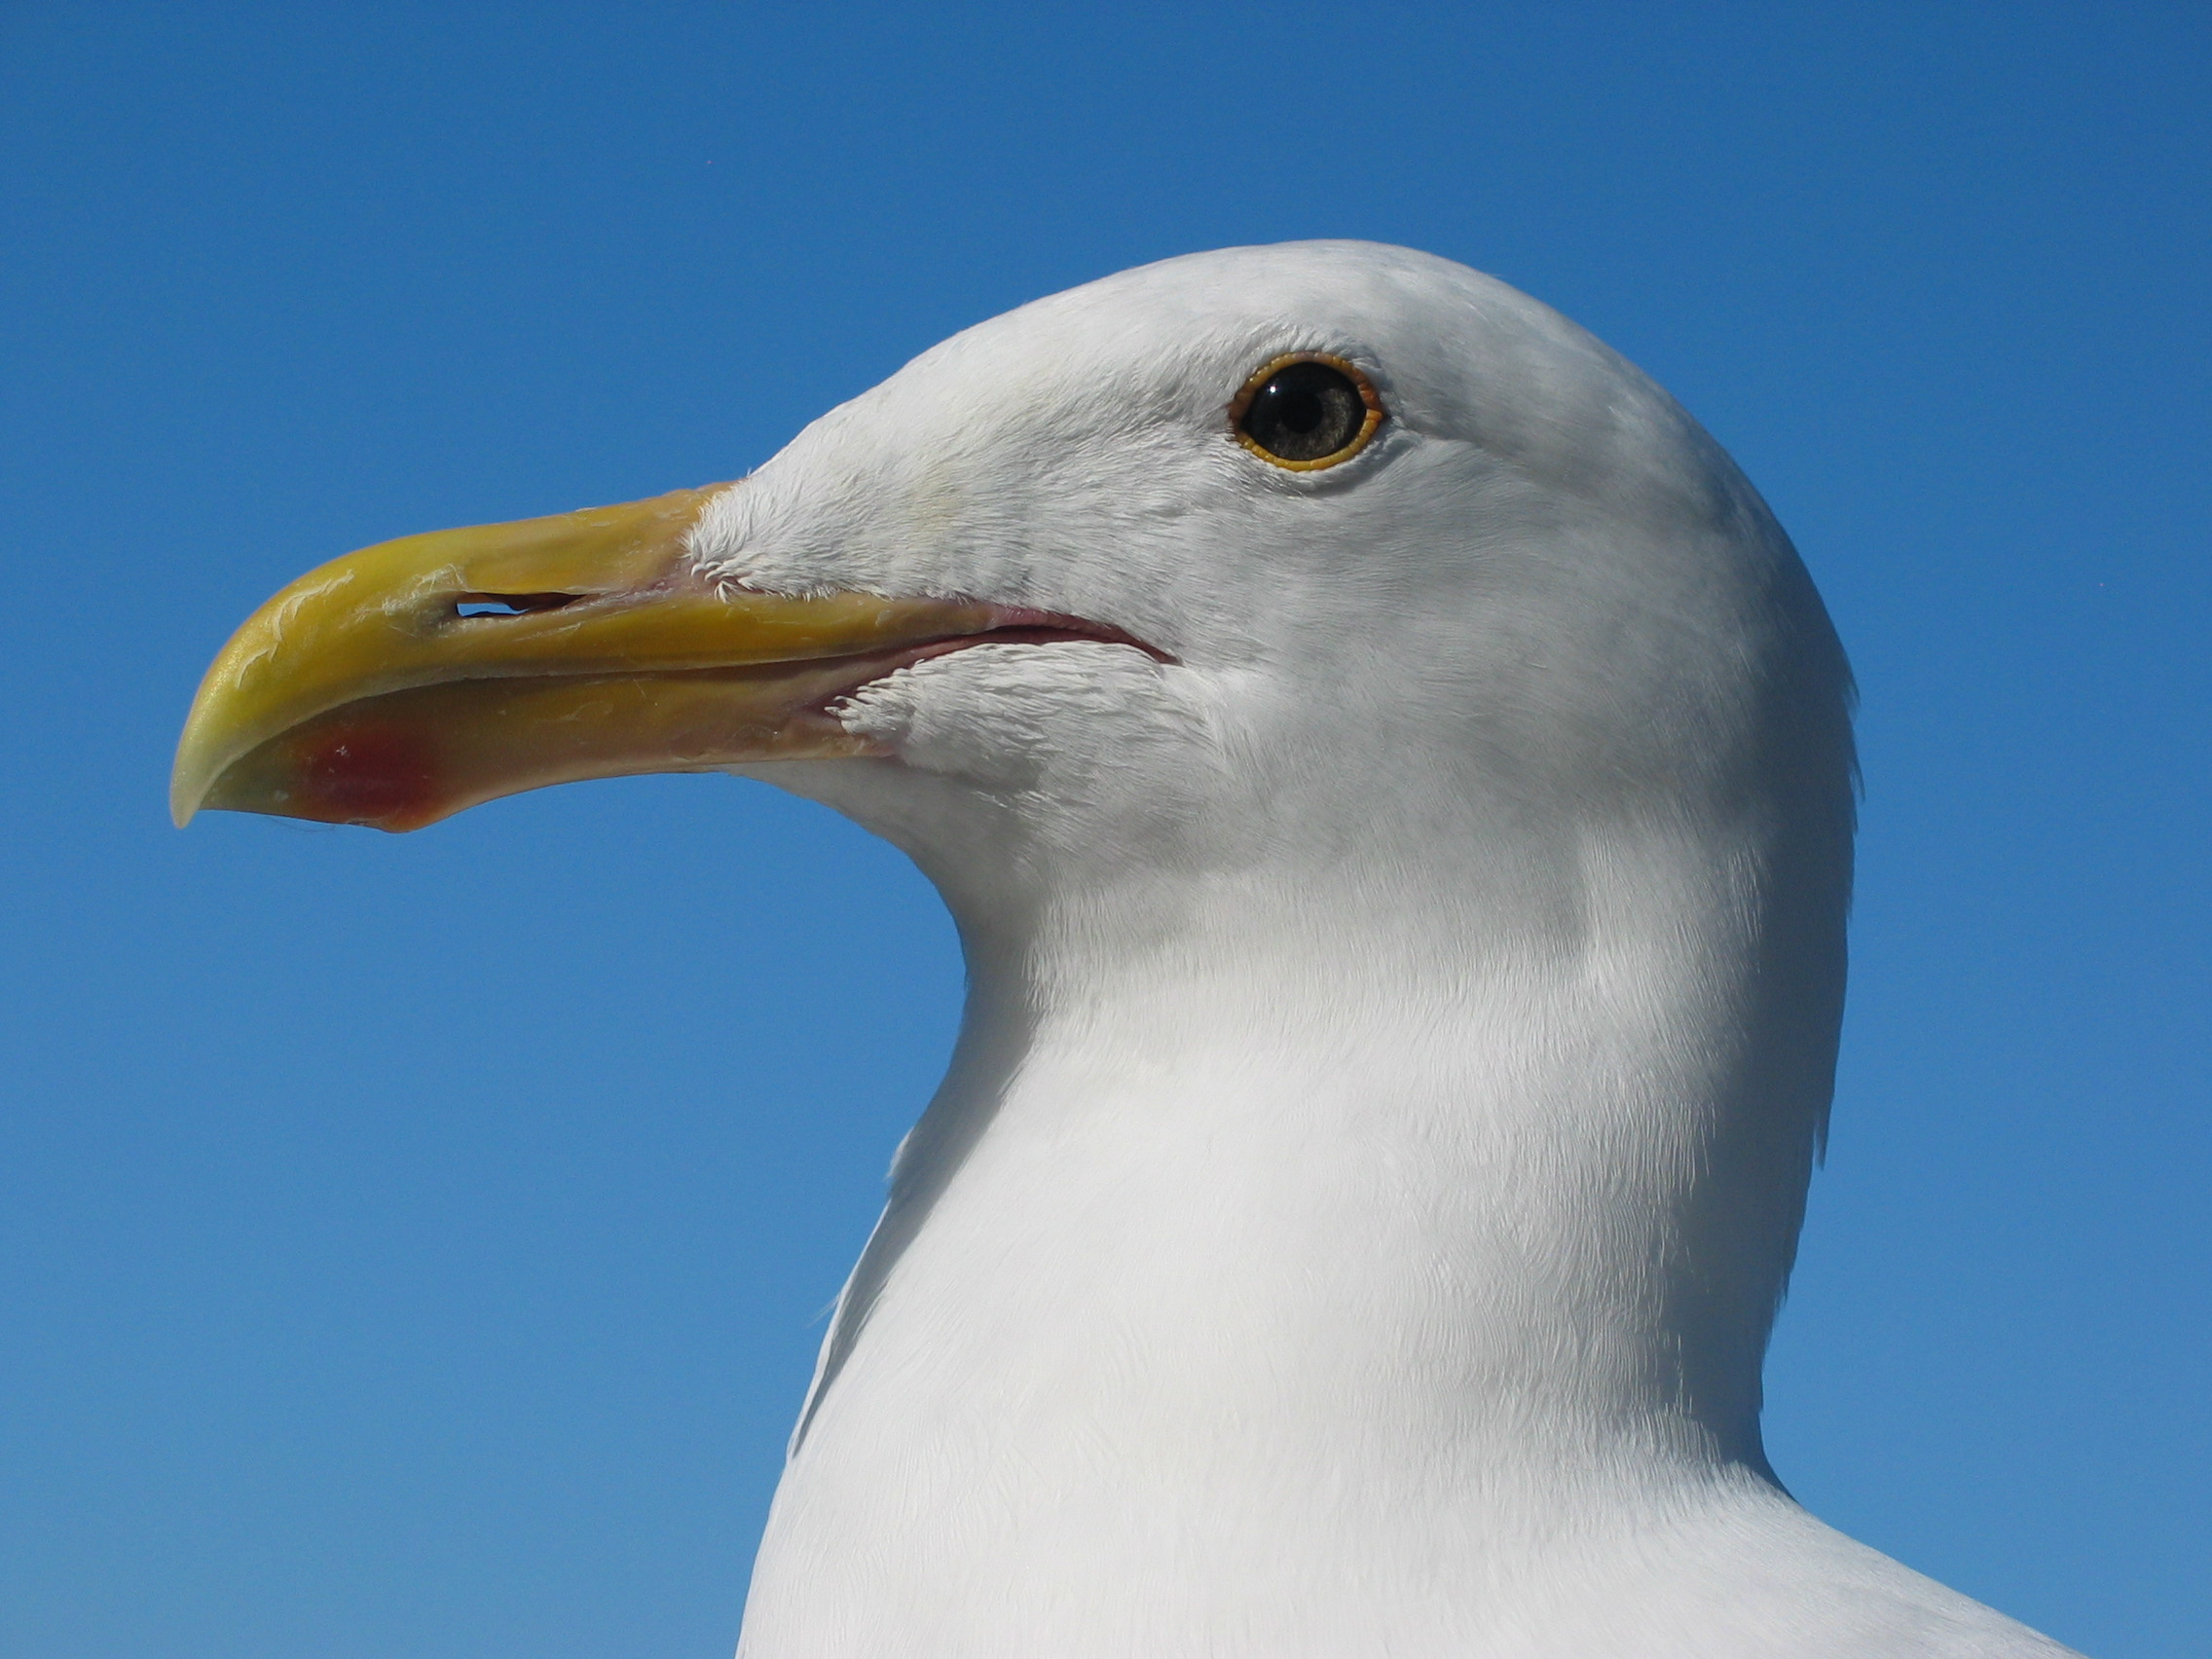
\includegraphics[width=0.5\textwidth]{images/gull}	
\end{figure}


% plusieurs figures côtes à côtes 
% voir : http://blog.pengyifan.com/the-best-way-to-place-figures-side-by-side-in-latex/
\begin{figure}
	\centering
	
  	\begin{subfigure}[b]{0.4\textwidth}
    		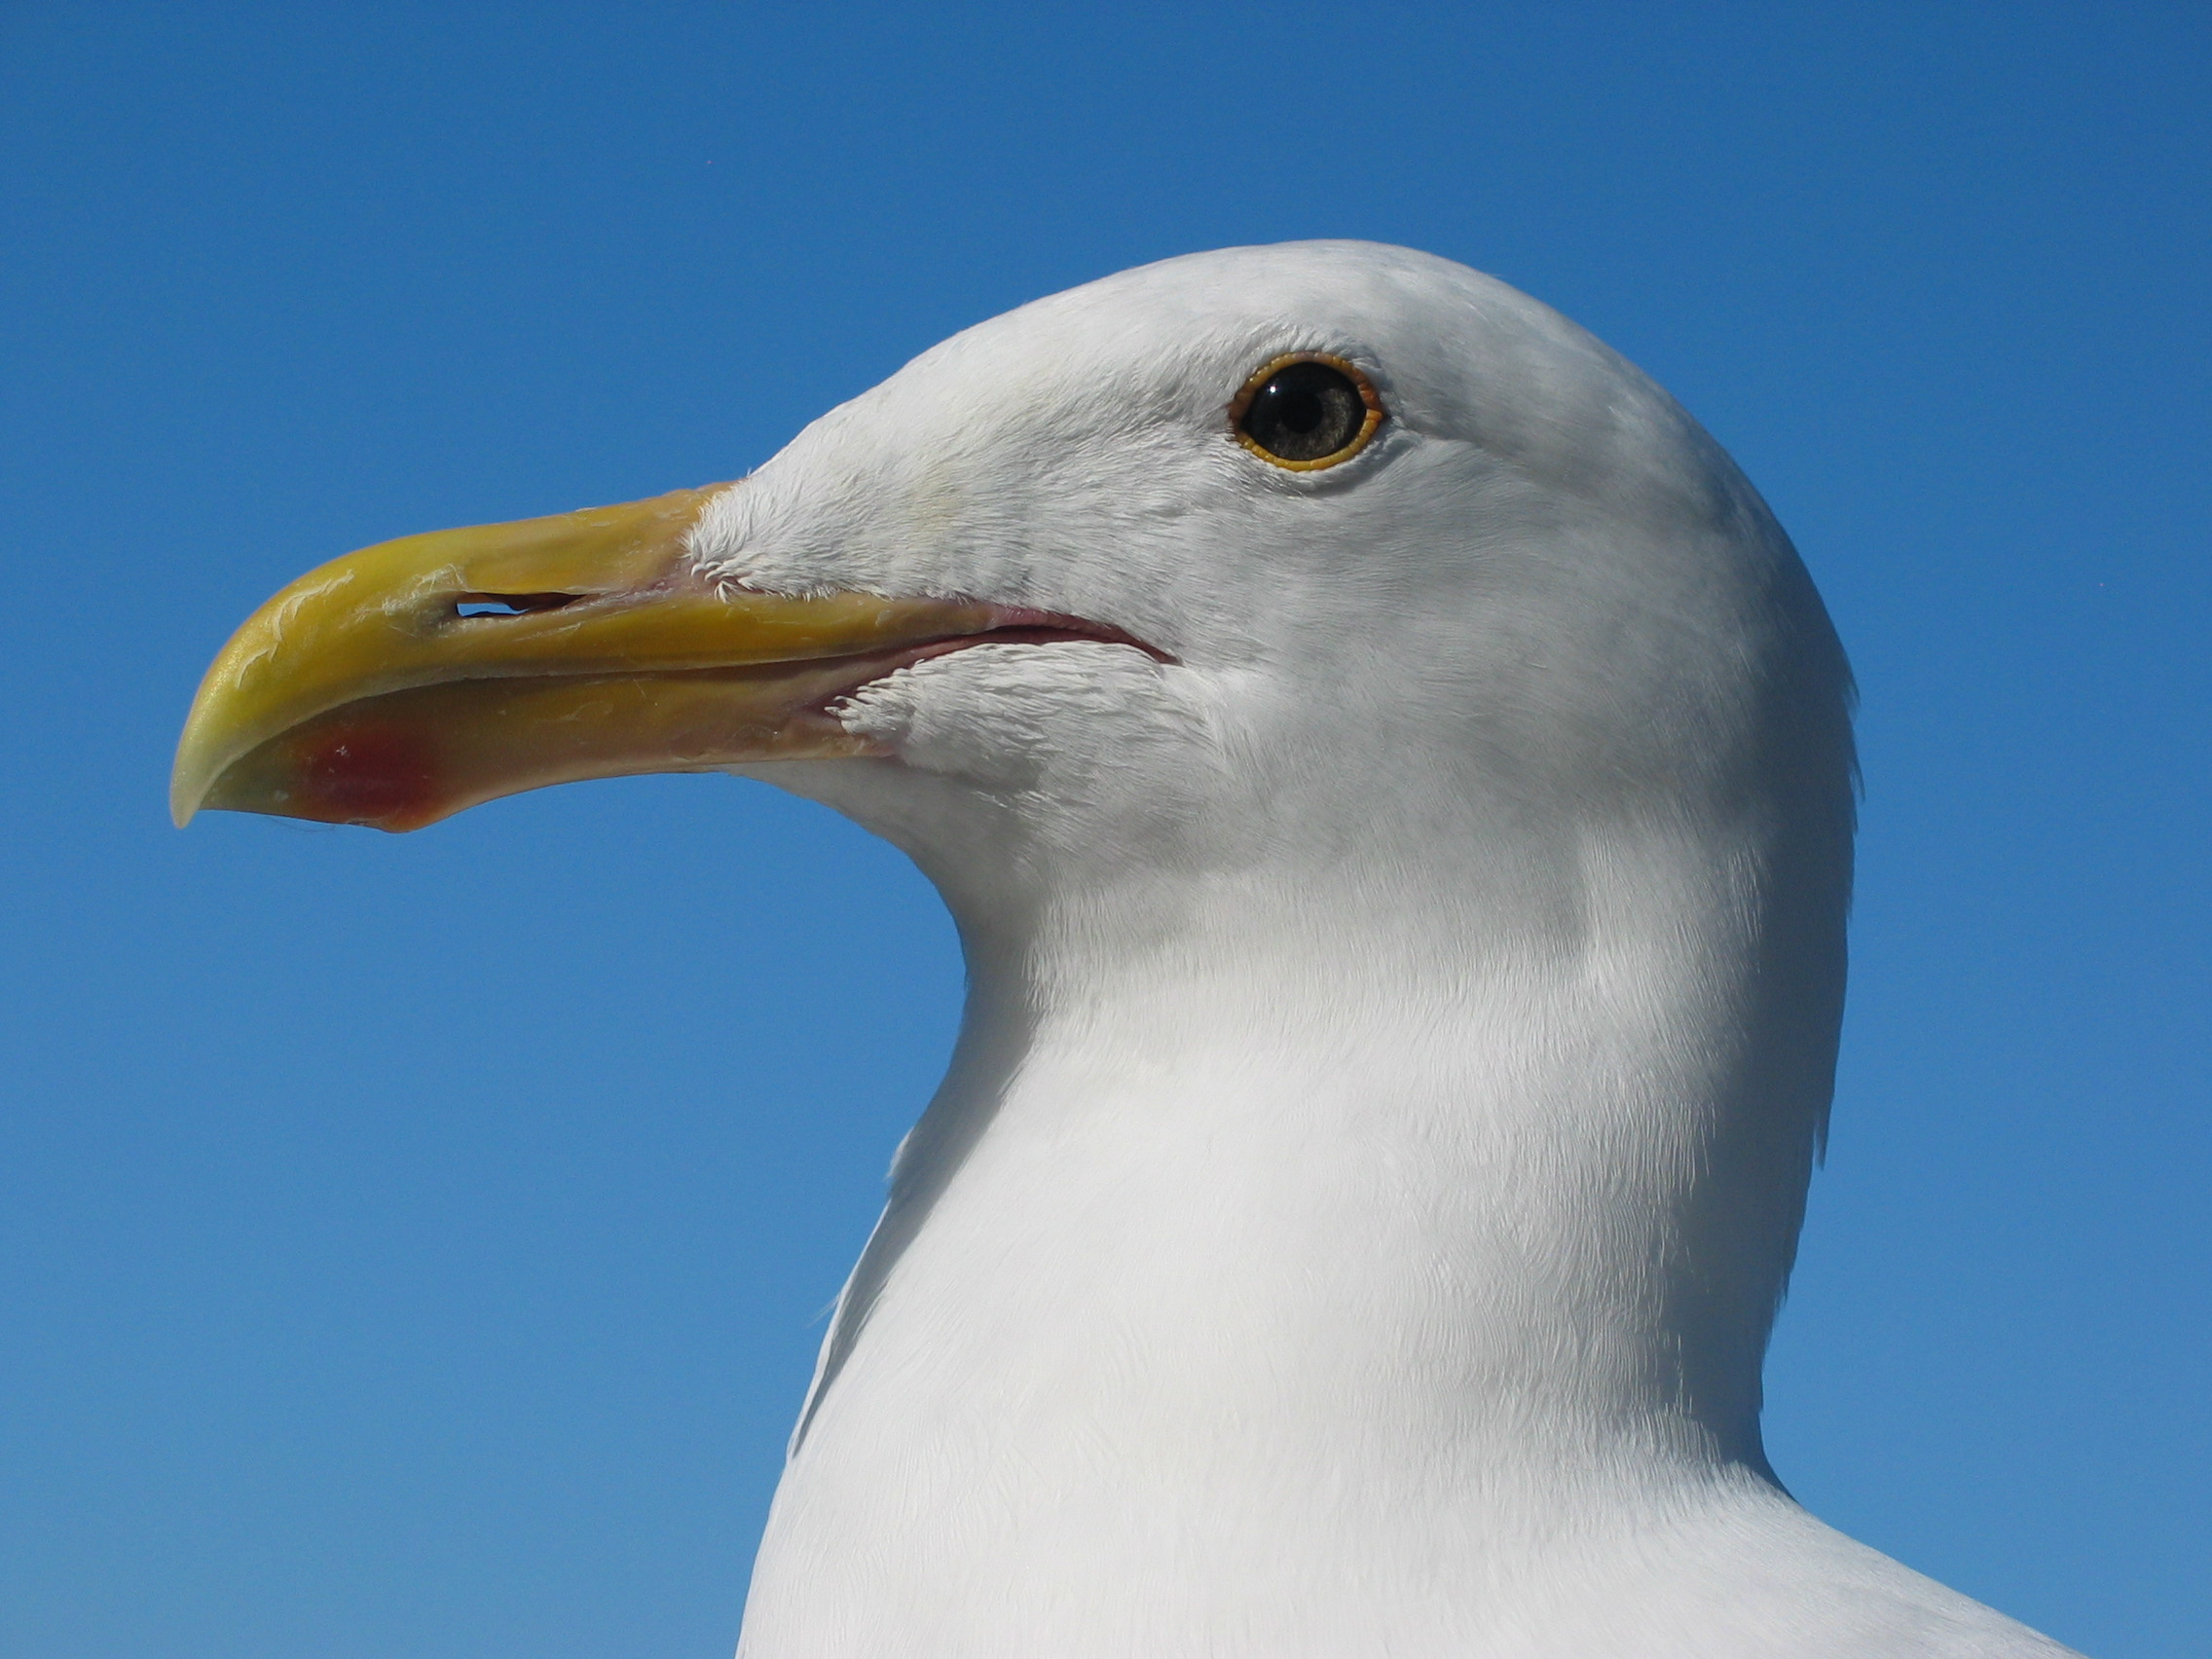
\includegraphics[width=\textwidth]{images/gull}
    		\caption{Picture 1}
    		\label{fig:1}
  	\end{subfigure}
  	\begin{subfigure}[b]{0.4\textwidth}
    		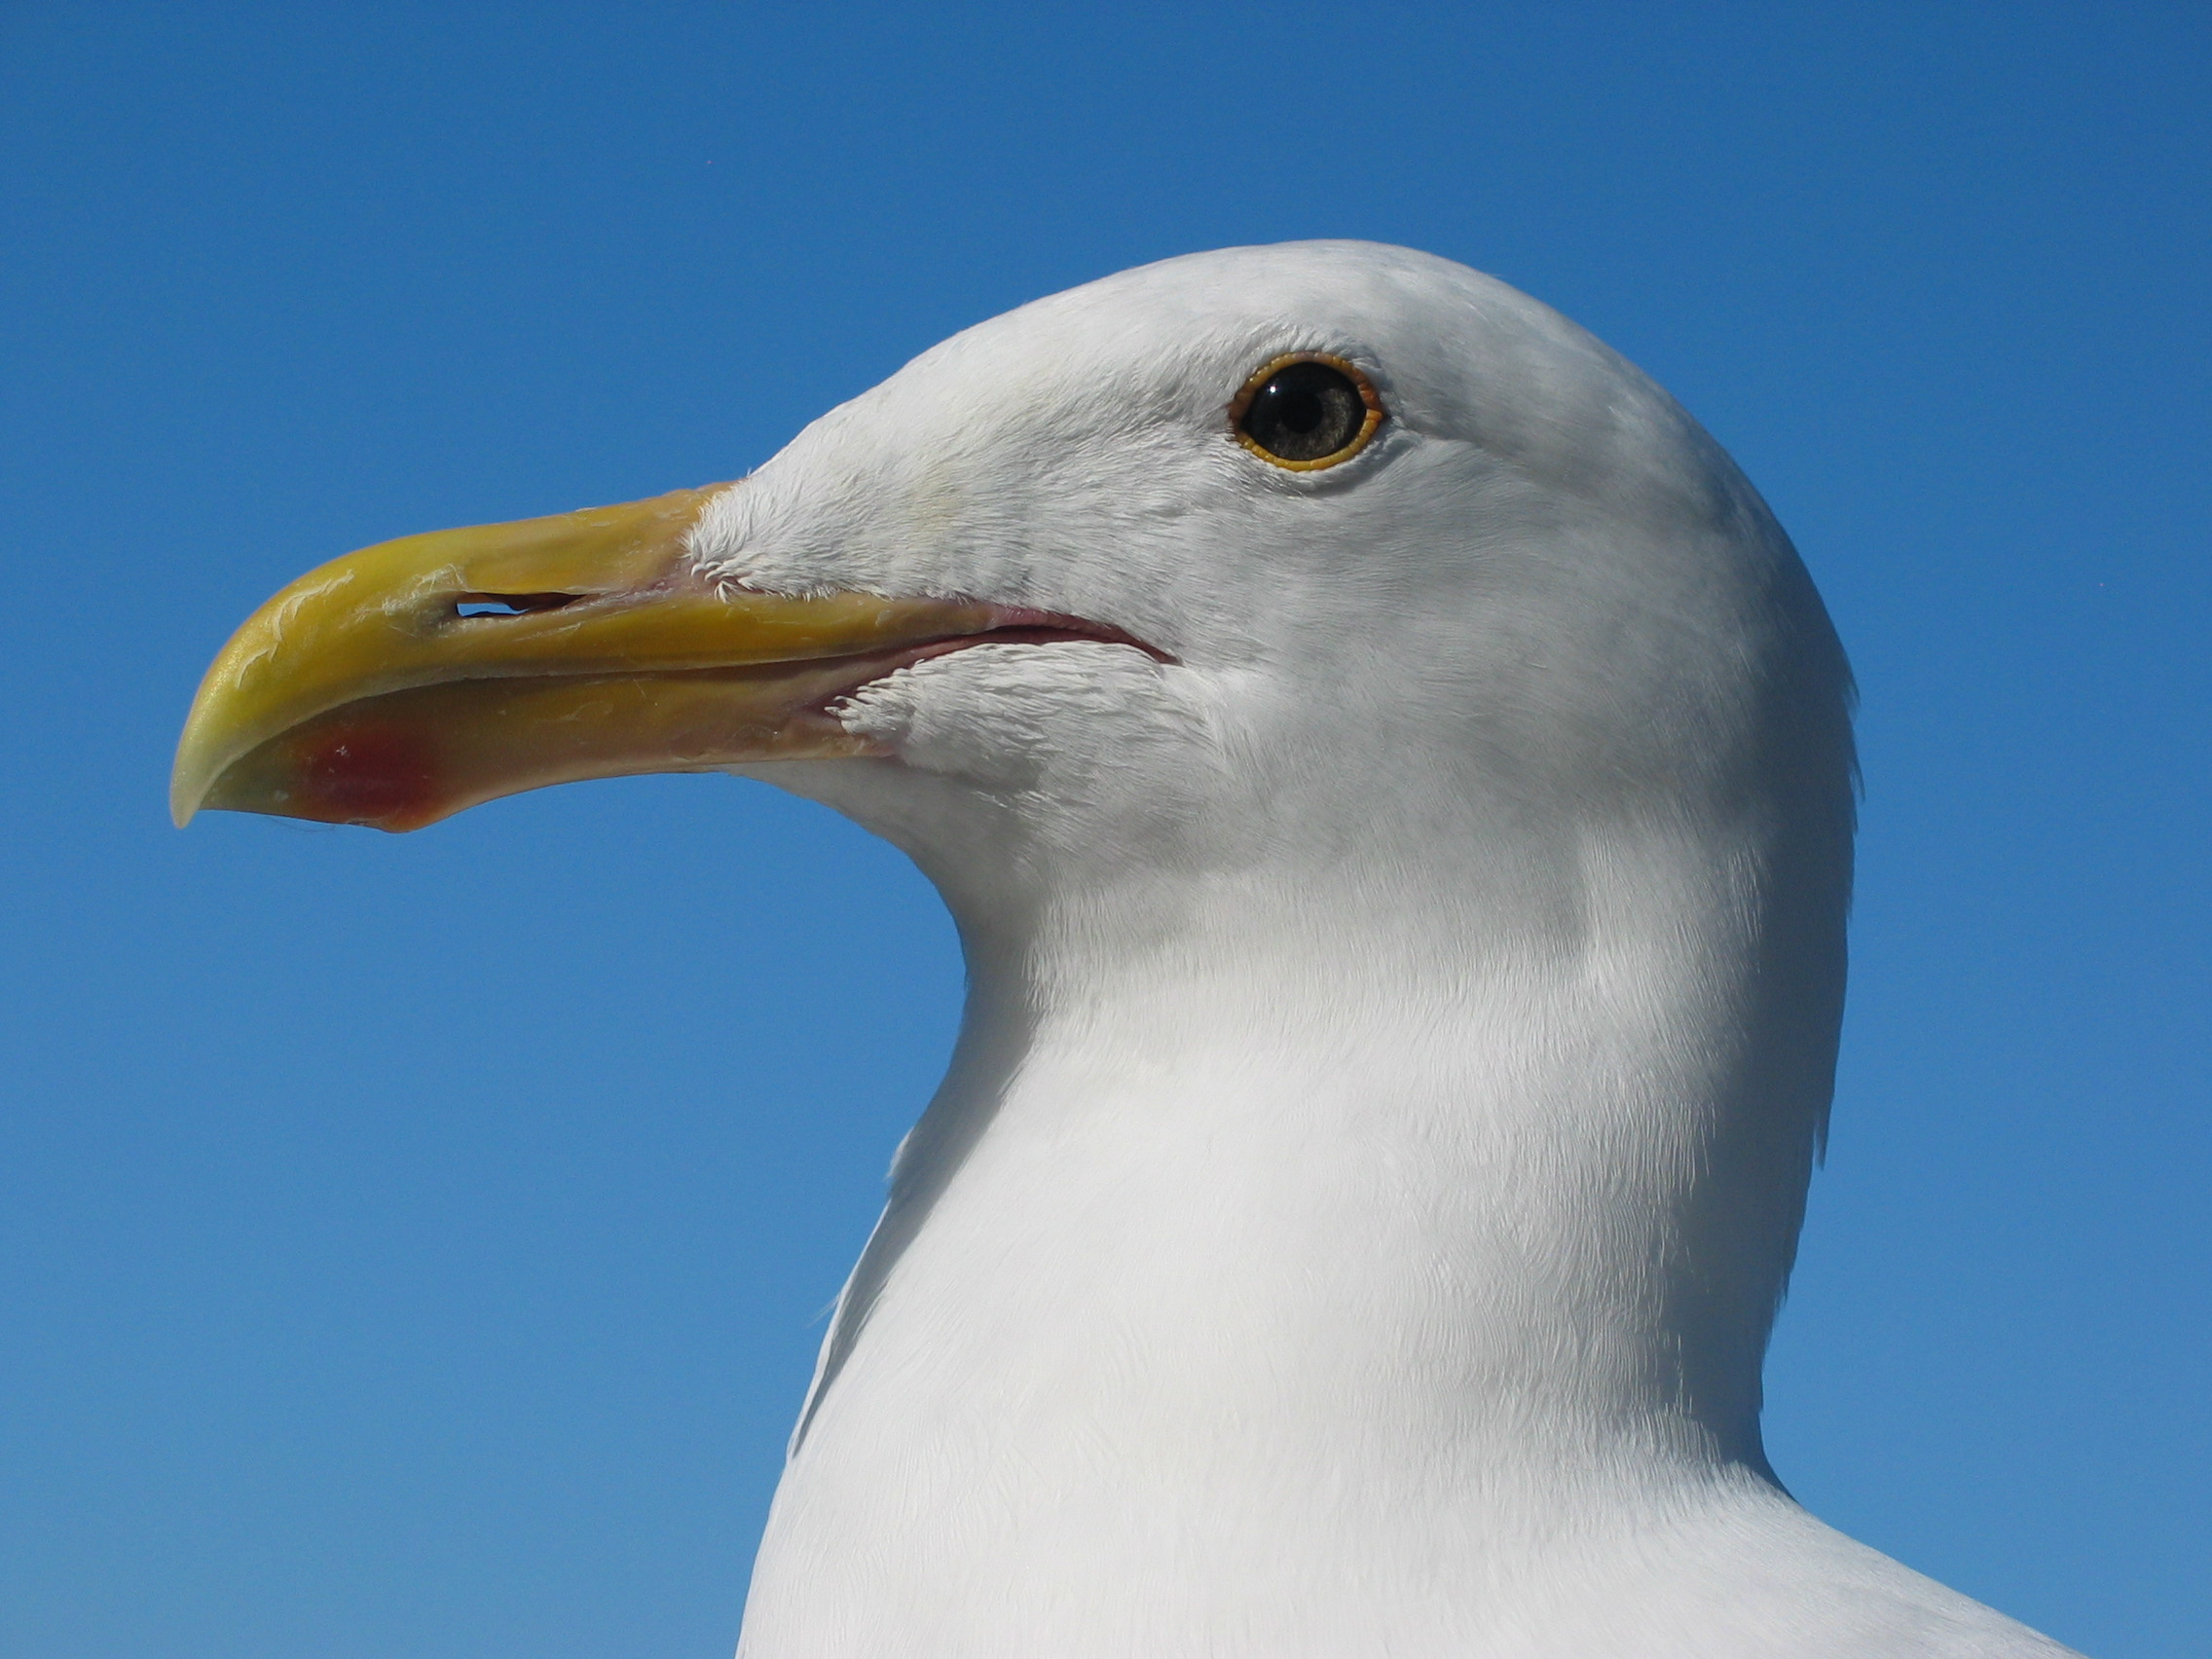
\includegraphics[width=\textwidth]{images/gull}
    		\caption{Picture 2}
    		\label{fig:2}
  	\end{subfigure}
	
	\caption{global}
\end{figure}



%%%%%%%%%%%%%%%%%%%%%%%%%%%%%%%%%%%%%%%%%%%%

  \begin{figure}
      %\centering
      
        \begin{subfigure}[b]{1\textwidth}
            \parbox[b]{.5\linewidth}{
            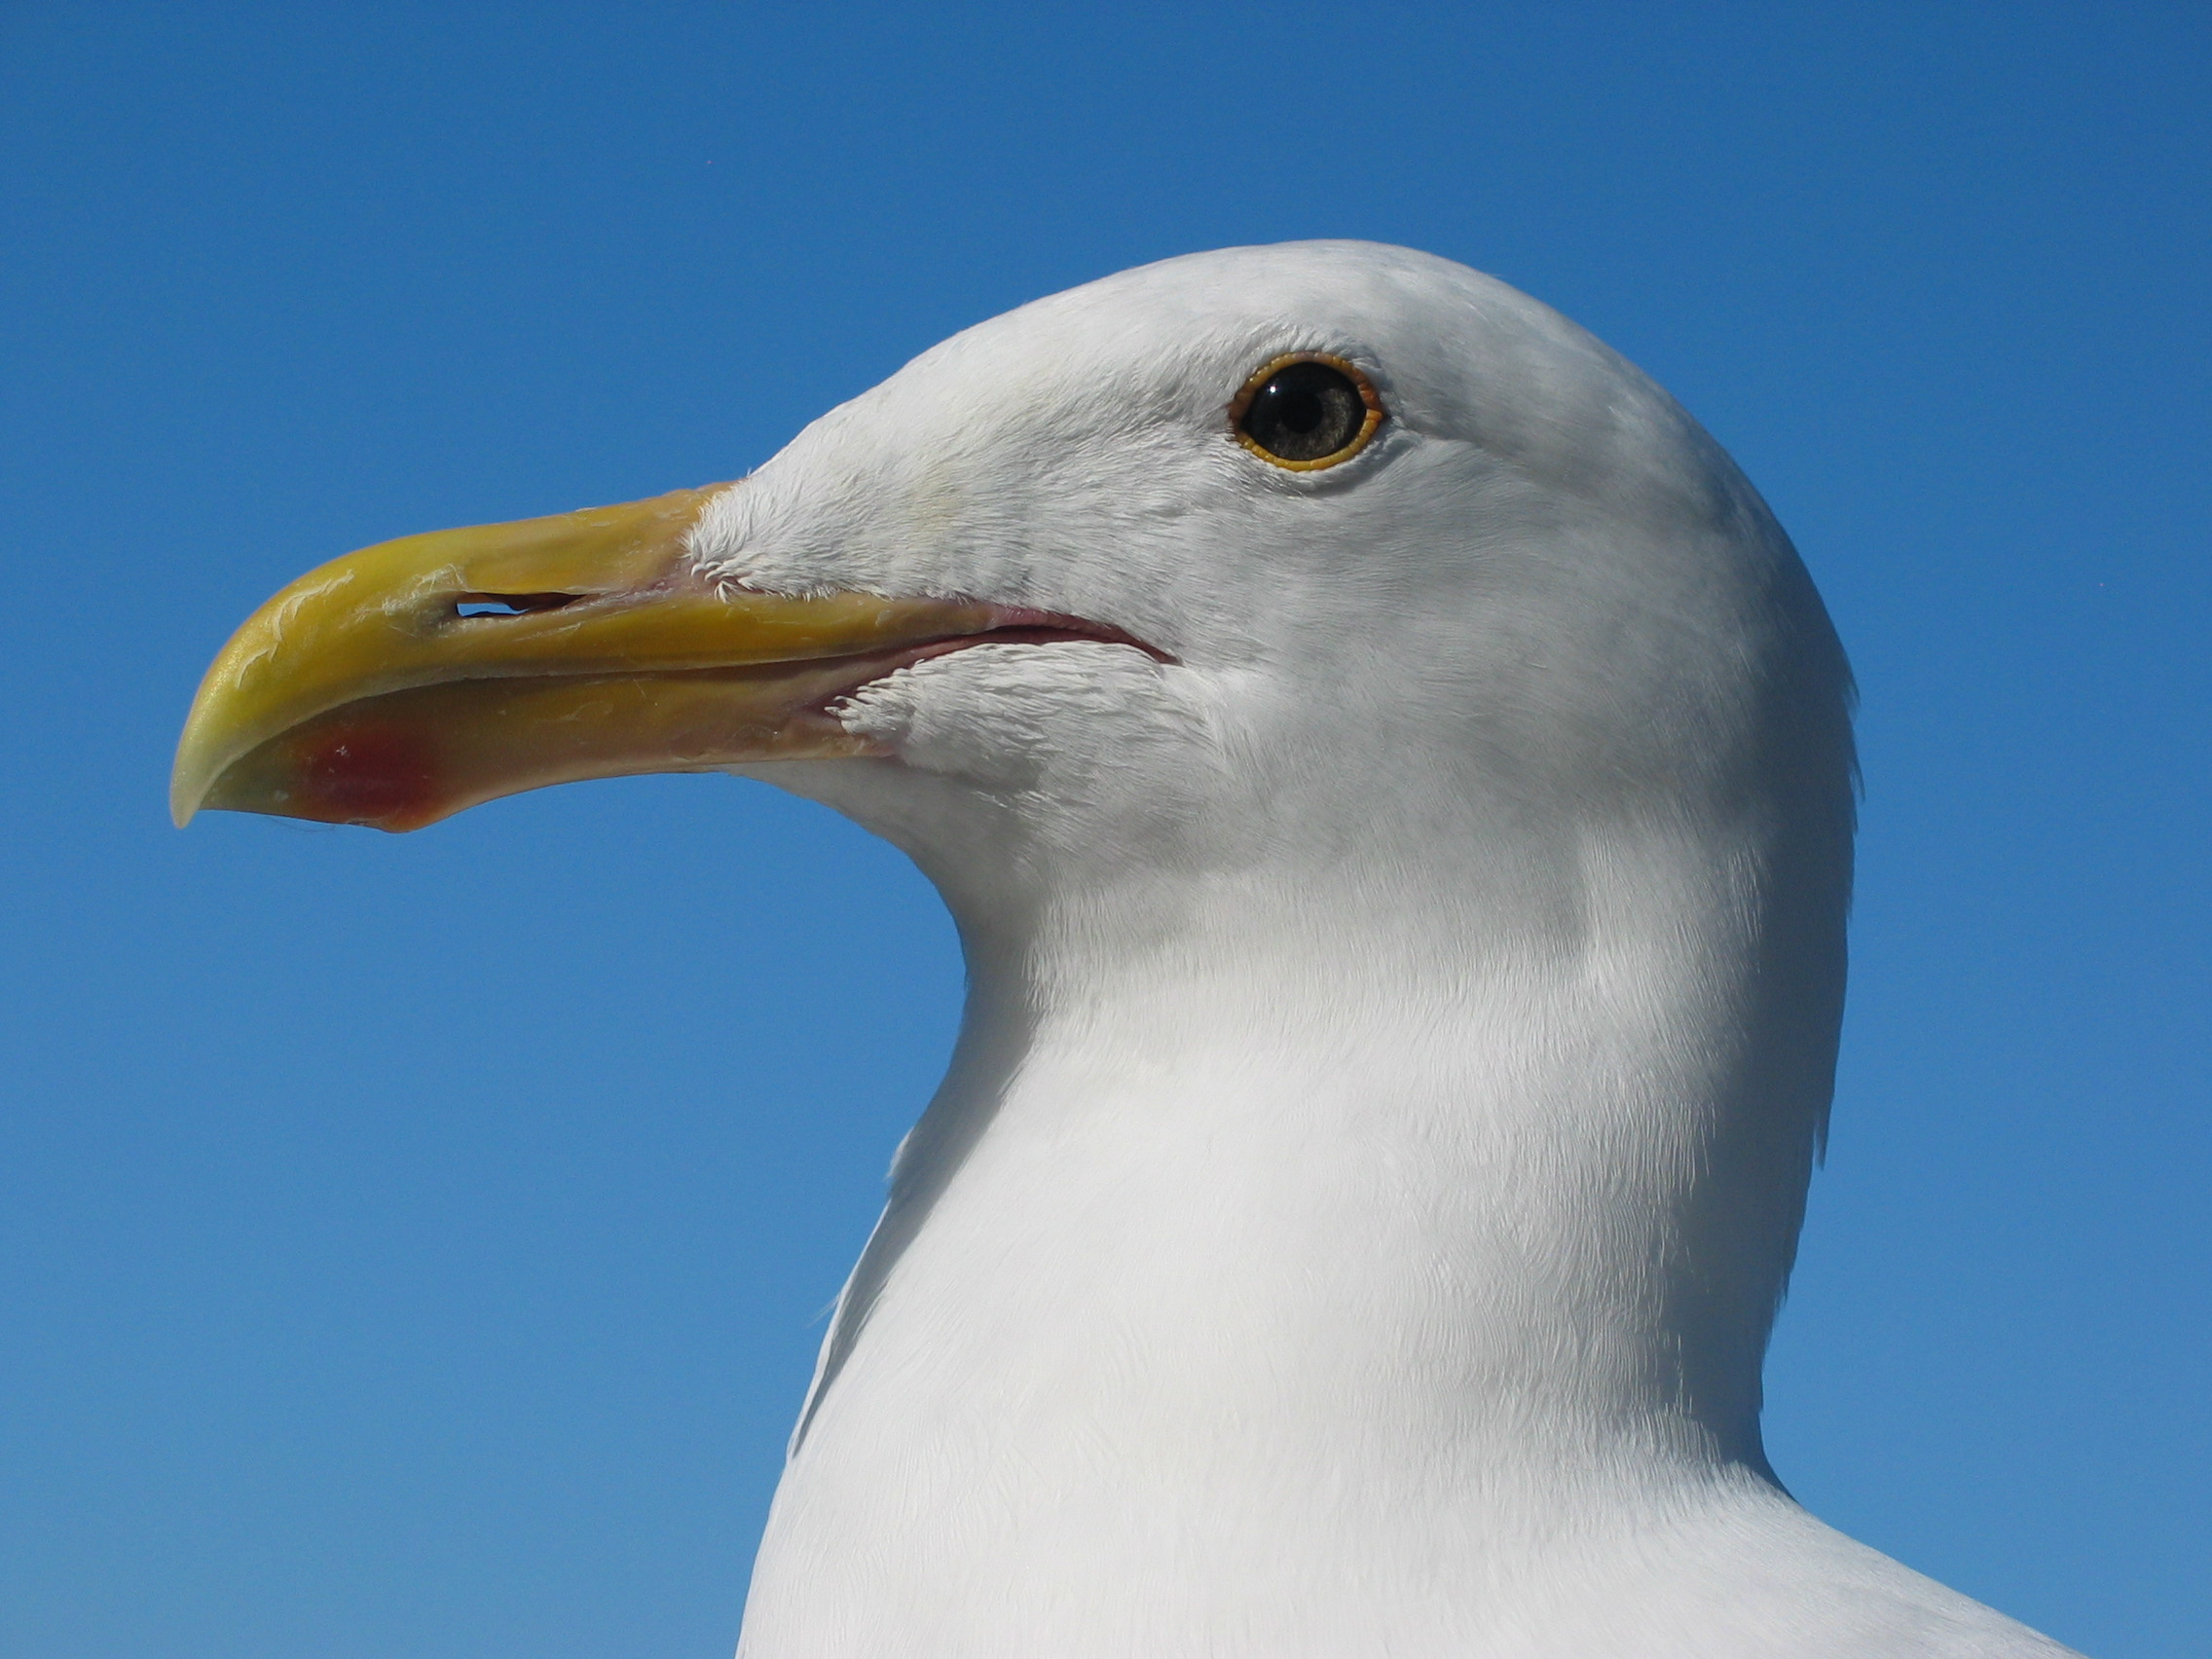
\includegraphics[height=0.2\textwidth]{images/gull}
            }
            \parbox[b]{.4\linewidth}{
                \caption{Clappr}
            }
        \end{subfigure}
        
        \begin{subfigure}[b]{1\textwidth}
            \parbox[b]{.5\linewidth}{
                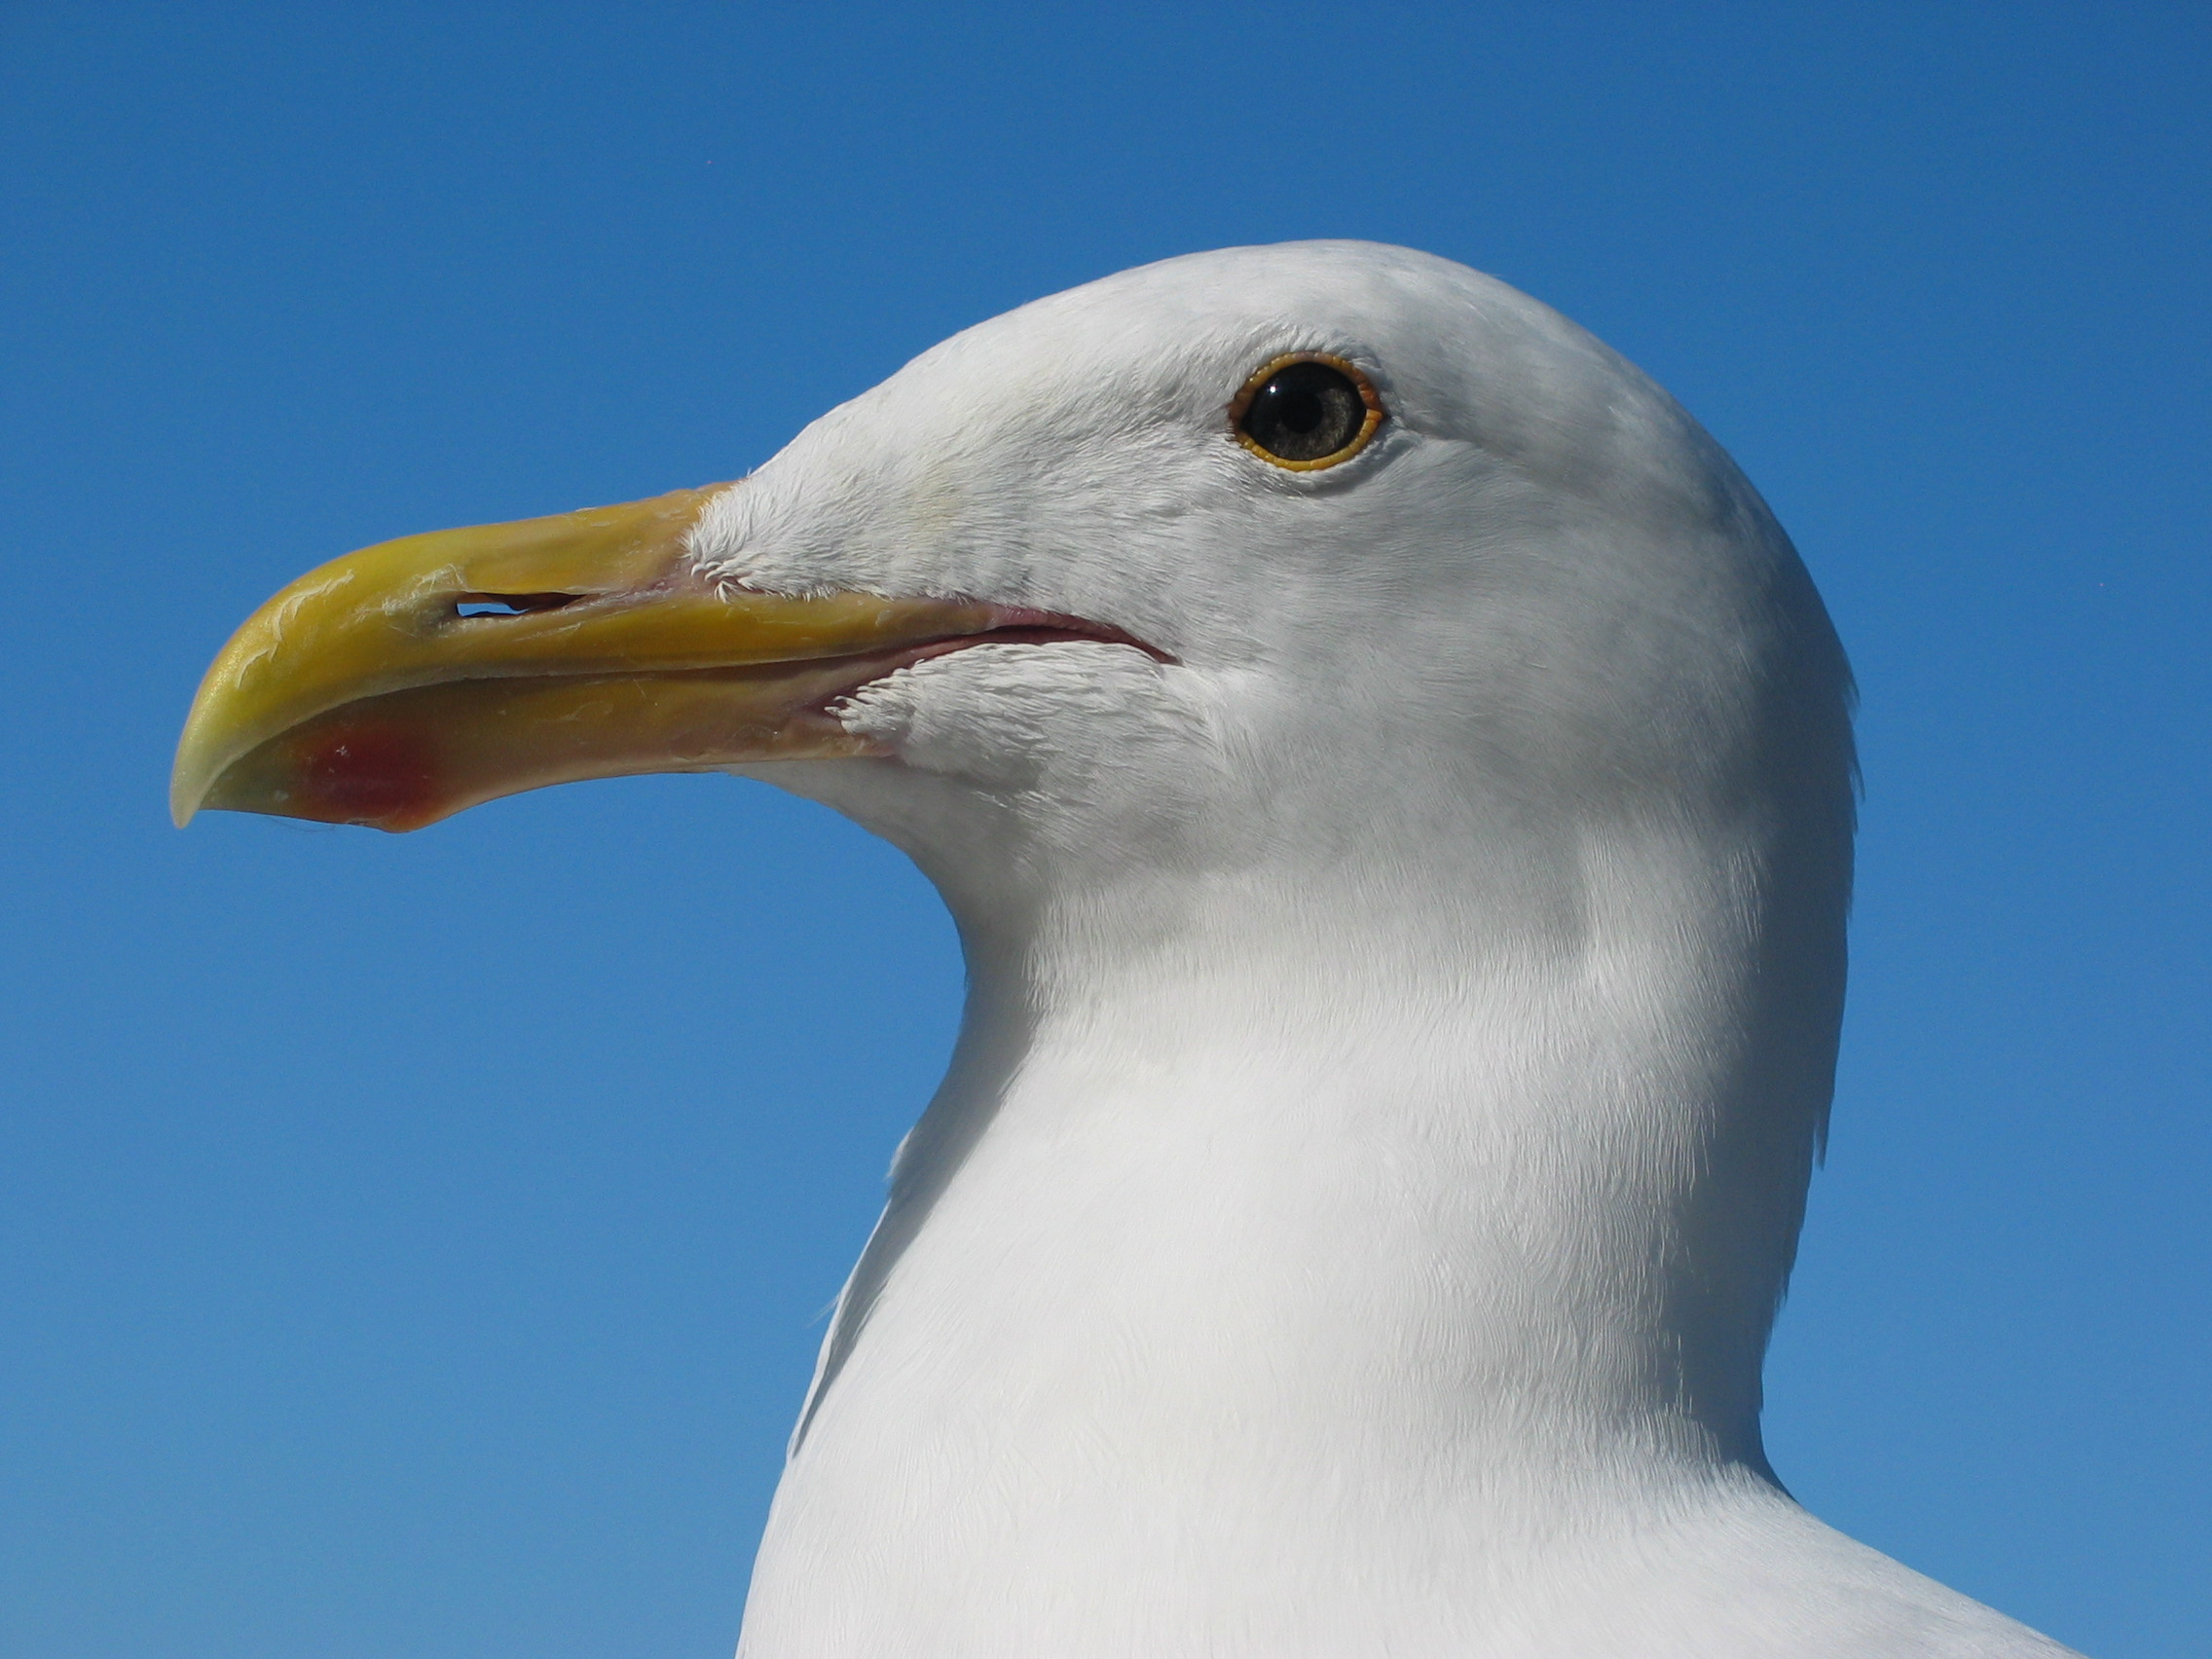
\includegraphics[height=0.2\textwidth]{images/gull}
            }
            \parbox[b]{.4\linewidth}{
                \caption{DashEB 1.0}
            }
        \end{subfigure}
        
        \begin{subfigure}[b]{1\textwidth}
            \parbox[b]{.5\linewidth}{
                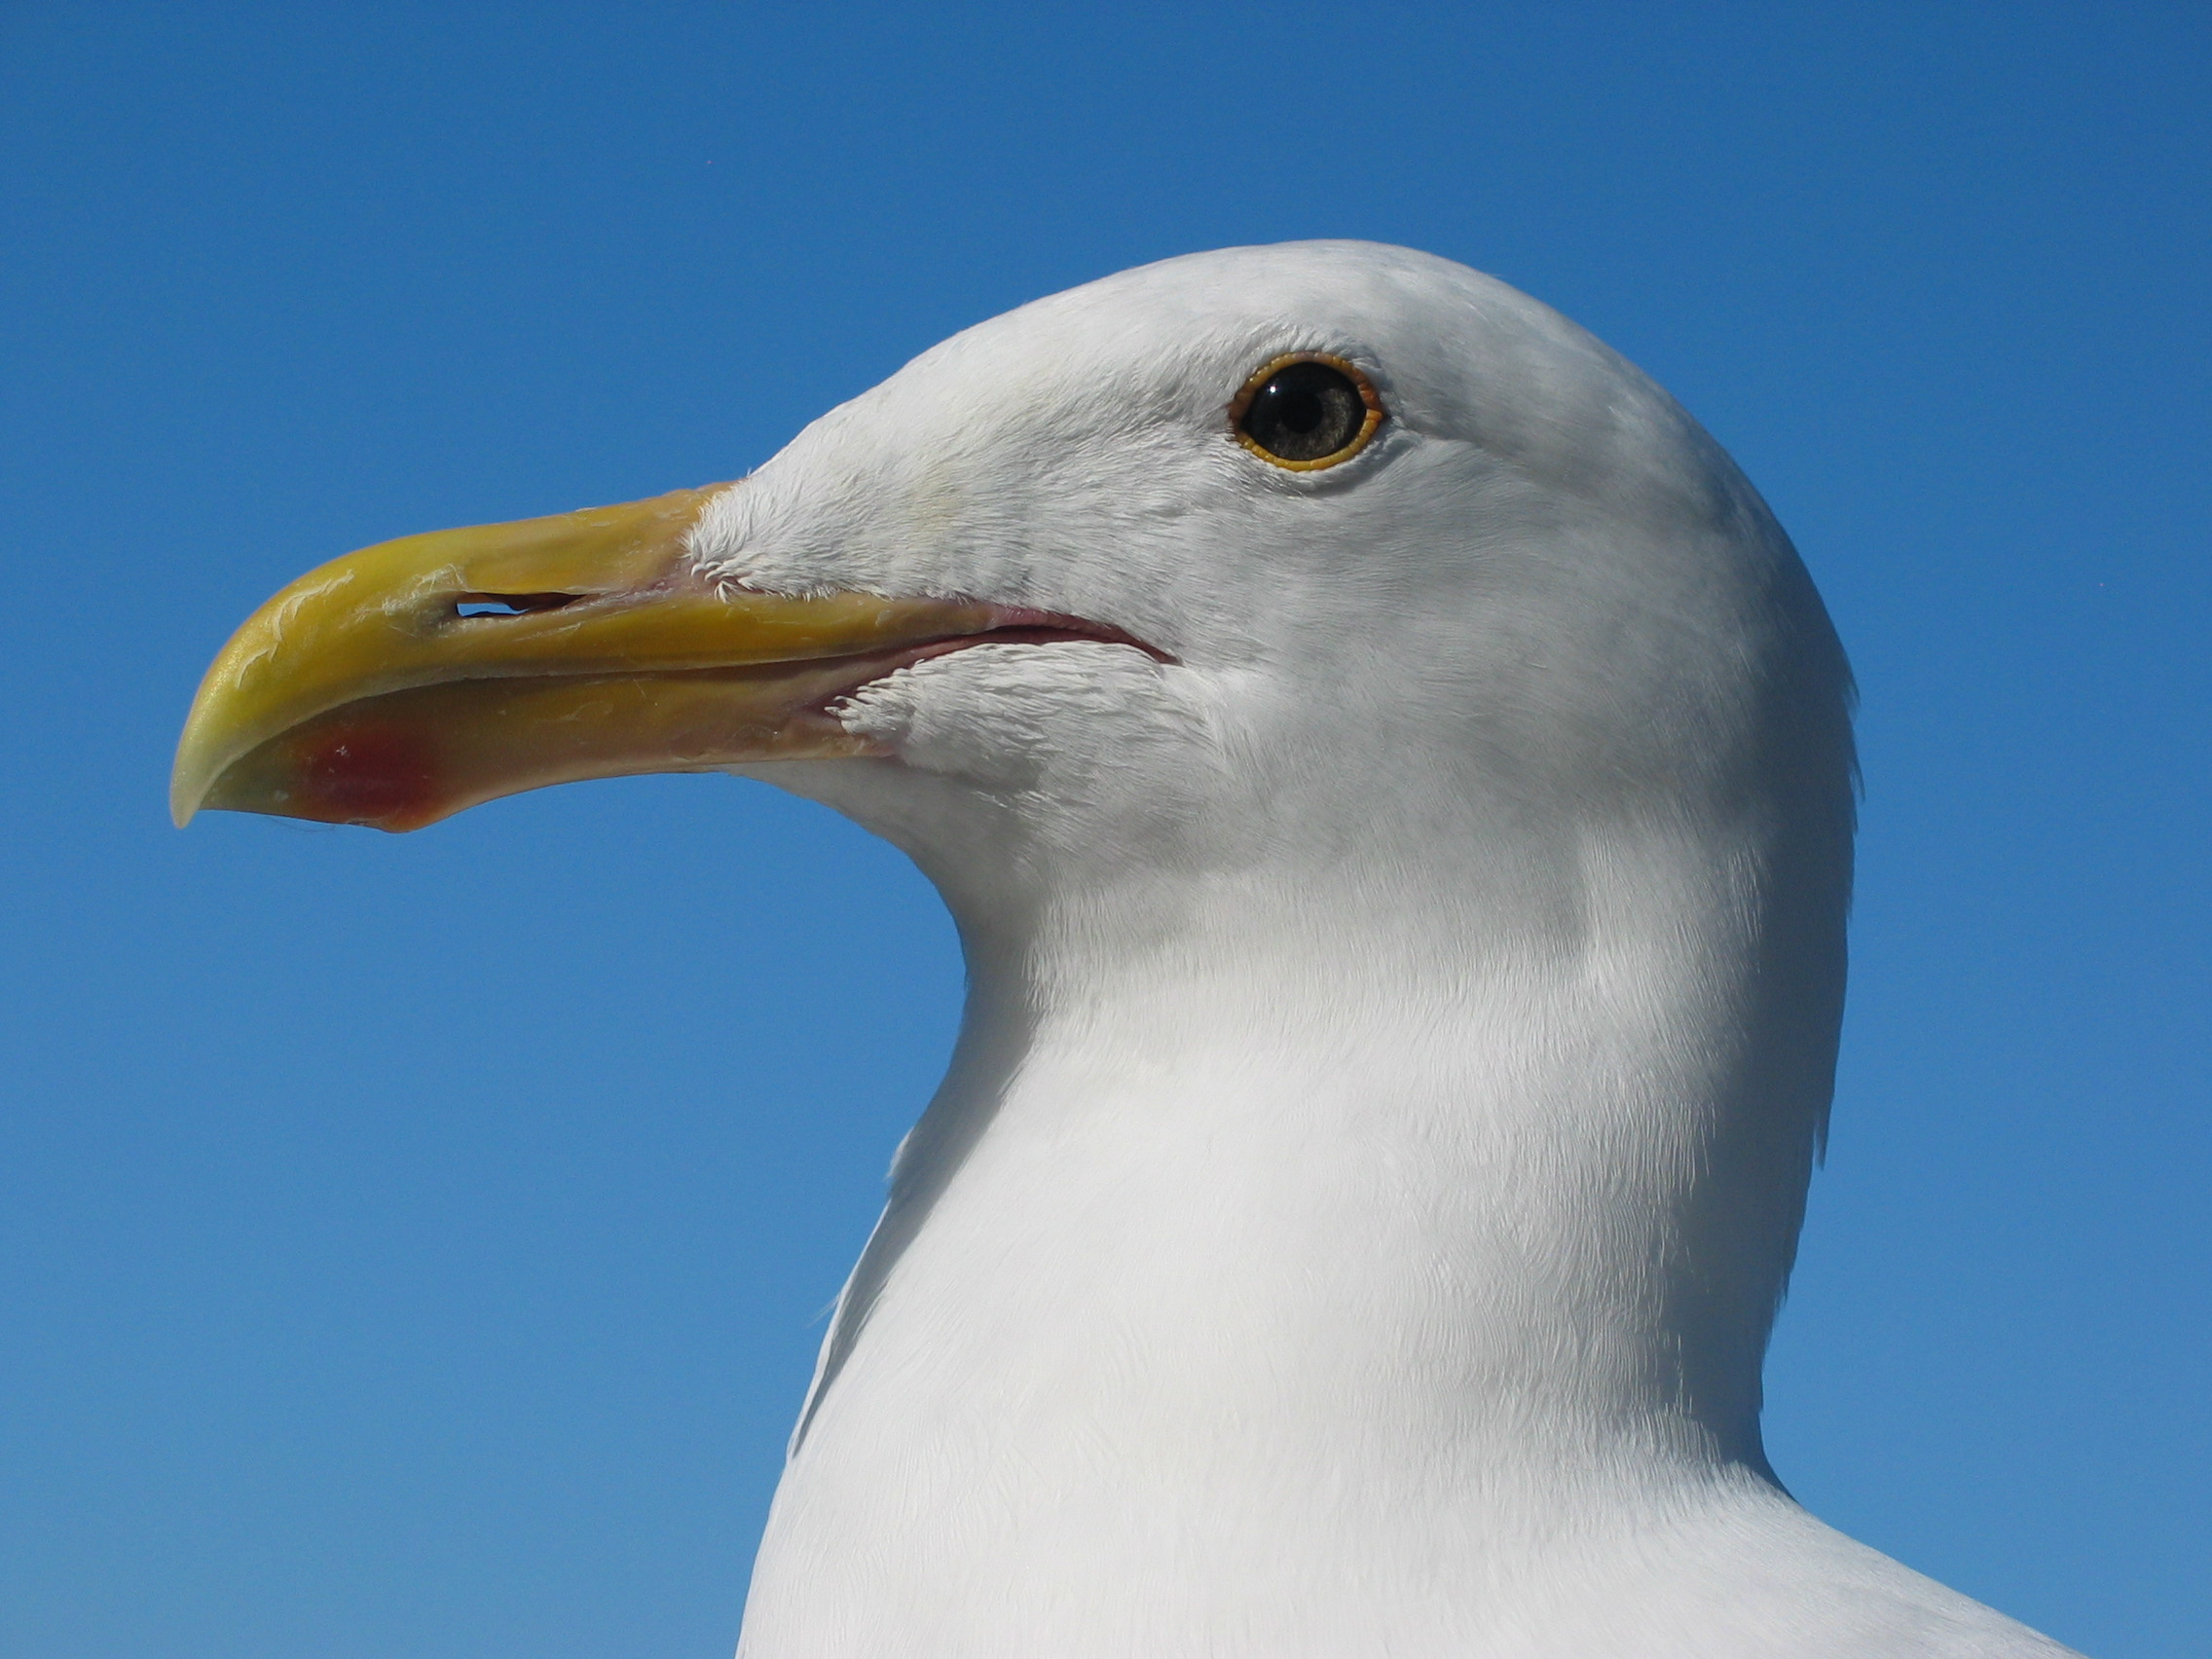
\includegraphics[height=0.2\textwidth]{images/gull}
            }
            \parbox[b]{.4\linewidth}{
                \caption{DashEB 2.0}
            }
        \end{subfigure}
      
      \caption{diffusion VOD}
    \end{figure}





\section{Les notes de bas de page / footnotes}

Voici une note de bas de page\footnote{une note de bas de page}. En voici plusieurs à la fois\footnote{1 ; 2}. test \multfootnote{un;deux;trois}. Ceci est aussi possible mais ne marche pas bien avec les '.', donc ne pas le faire \footnote{première}\footnote{deuxième}.

~~

Des footnotes dans un tableau 

\begin{savenotes}
%\begin{table}[H]
%	\centering
	\begin{tabular}{c} 
		\toprule
     	un tableau \footnote{une footnote dans un tableau, mis en bas de la page} \\
		\bottomrule
	\end{tabular}
%	\caption{Avec des footnotes en bas de page}
%\end{table}
\end{savenotes}

Des footnotes en dessous d'un tableau 


%\begin{table}[H]
%	\centering
	\begin{minipage}{3cm}
	\begin{tabular}{lcc}
        \toprule
        A & 1 & 2 \footnote{une footnote en dessous du tableau} \\
        \bottomrule
    \end{tabular}
	\end{minipage}
%	\caption{Footnotes juste en dessous de moi}
%\end{table}



%

\section{Maths}
% http://dalissier.perso.math.cnrs.fr/pdf/latex/chapitre4.pdf

\subsection{environnements}

\subsubsection{en ligne}

En lignes : $math$

Encore en ligne : 
\begin{math}
	math
\end{math}


Si l'équation est coupée entre deux lignes, utiliser "mbox" \mbox{$f(x)=12$}


\subsubsection{en centrée}

Équation centrée : 

\begin{displaymath}
	math centree
\end{displaymath}


Équation centrée et numérotée :

\begin{equation}
	\label{eq:equation}
	math centree
\end{equation}


Utilisation des références possibles : \ref{eq:equation}.


\subsection{opérations possibles}

$variable_{indice}$

$variable^{exposant}$

$\frac{nominateur}{denominateur}$

racine : $\sqrt{equation}$

racine n-ieme : $\sqrt[n]{equation}$

\subsubsection{Opérateurs}


\begin{itemize}
	\item somme $\sum$
	\item produit $\prod$
	\item intégrale $\int$
	\item grande intersection $\bigcap$
	\item grande union $\bigcup$
	\item intersection $\cap$
	\item union $\cup$
	\item diviser $\div$
	\item multiplier $\times$
	\item point $\cdot$
	\item $\backslash$
\end{itemize}

Opérateurs binaires $\leq \le \geq \ge \equiv \sim \simeq \approx \perp \subset \in \not\in \not\subset \not= \not\equiv$

Un exemple : $resultat = \sum_{x=0}^{10} x$


$\displaystyle\sum\nolimits_{i=1}^n $

vecteur : $\overrightarrow{a}$

barre : $\overline{a}$

n fois : $\underbrace{a \times \dots \times a}_{n fois}$

grandes parenthèses $\left( x + \frac{1}{2} \right)$

marches avec tous les autres aussi $\left\{ \left [ \left(  \right) \right] \right\}$


\subsection{fonctions mathématiques}

\begin{itemize}
	\item cos : $\cos x$
	\item sin : $\sin x$
	\item tan : $\tan x$
	\item lim : $\lim$
	\item min : $\min$
	\item ln : $\ln $
	\item exp : $\exp x$
	\item log : $\log x$
	\item arg : $\arg x$
	\item max : $\max$
	\item modulo : $a \bmod b$
\end{itemize}


\subsection{symboles}

\subsubsection{les formats}

Caractères 
\begin{itemize}
	\item $\mathrm{romain}$
	\item $\mathit{italique}$
	\item $\mathbf{gras}$
	\item $\mathcal{ABCDEFGHIJKLMNOPQRSTUVWXYZ}$
	\item $\mathbb{ABCDEFGHIJKLMNOPQRSTUVWXYZ}$
\end{itemize}


\subsubsection{lettres grecques}

$\alpha$ $\beta$ $\gamma$ $\delta$ $\epsilon$ $\varepsilon$ $\theta$ $\lambda$ $\mu$ $\pi$ $\rho$ $\sigma$ $\phi$ $\varphi$ $\psi$ $\omega$ $\Gamma$ $\Sigma$ $\Psi$ $\Delta$ $\Omega$ $\Pi$ $\Phi$



\subsubsection{autres symboles}

\begin{itemize}
	\item petits points  $\dots$
	\item flèche droite  $\rightarrow$
	\item infini $\infty$
	\item cercle $\circ$
	\item vide $\emptyset$
	\item accolade $\lbrace \rbrace$
\end{itemize}

\subsection{tableaux et matrices}

\begin{equation}
	\begin{array}{lcc}
	x & = & 3 \\
	y & : & 4	
	\end{array}
\end{equation}


\gls{mot} \cite{bib:reinforcement_learning_in_robotics}

\layout


\printbibliography 
\listoffigures 
\listoftables 
\listoflistings 
\printglossary 


%\newpage
%\pagenumbering{Roman}	% numérotation .I, .II, .III
%\pagestyle{appendix}
%\appendix	% début des appendices, chapitre numéroté alphabétiquement


%\addcontentsline{toc}{part}{Annexes}
%\chaptermark{Annexes}
%\part*{Annexes}
%% pour ajouter les annexes dans la table des matières
\cleardoublepage	% évite les erreurs de numérotation
\phantomsection		% évite les erreurs de placement de lien


\addcontentsline{toc}{chapter}{Annexes}
\chapter*{Annexes}
\label{ch:annexes}
\chaptermark{Annexes}	% met "Annexes" en haut de page à droite










\end{document}